\section{Chrome Extension for Stack Overflow}
\label{sec:chrome}

In the purpose of helping with qualitative analysis, we build a Chrome extension for the Stack Overflow query code base and GitHub search code corpus. Figure \ref{fig:chrome} shows a screenshot of using the Chrome extension. The highlighted yellow snippet is the query method from SO, and on the right-hand side we present the ranked list of related code fragments from GitHub. The Chrome extension provides a clearer presentation of the query and the resulting related code in the process of manual evalutation.

The Chrome extension also demonstrates a real-life use scenario of getting related methods from GitHub for a SO snippet, thus serves as a proof of our concept of recommending related code fragments.
The real-life use scenario will be: suppose the user is searching on Stack Overflow for the question {\ttt how to unzip a folder in java}. The user locates the highlighted yellow snippet as the correct implementation of the query functionality. They are interested in learning the other methods that can be possibly added to their project along with the {\ttt unzip} method. So the user invokes searching on {\tool} and gets recommended related methods. They may investigate the recommended results and select to add a {\ttt zip} method to complete the functionalities of file manipulation. 

\begin{figure*}[!h]
	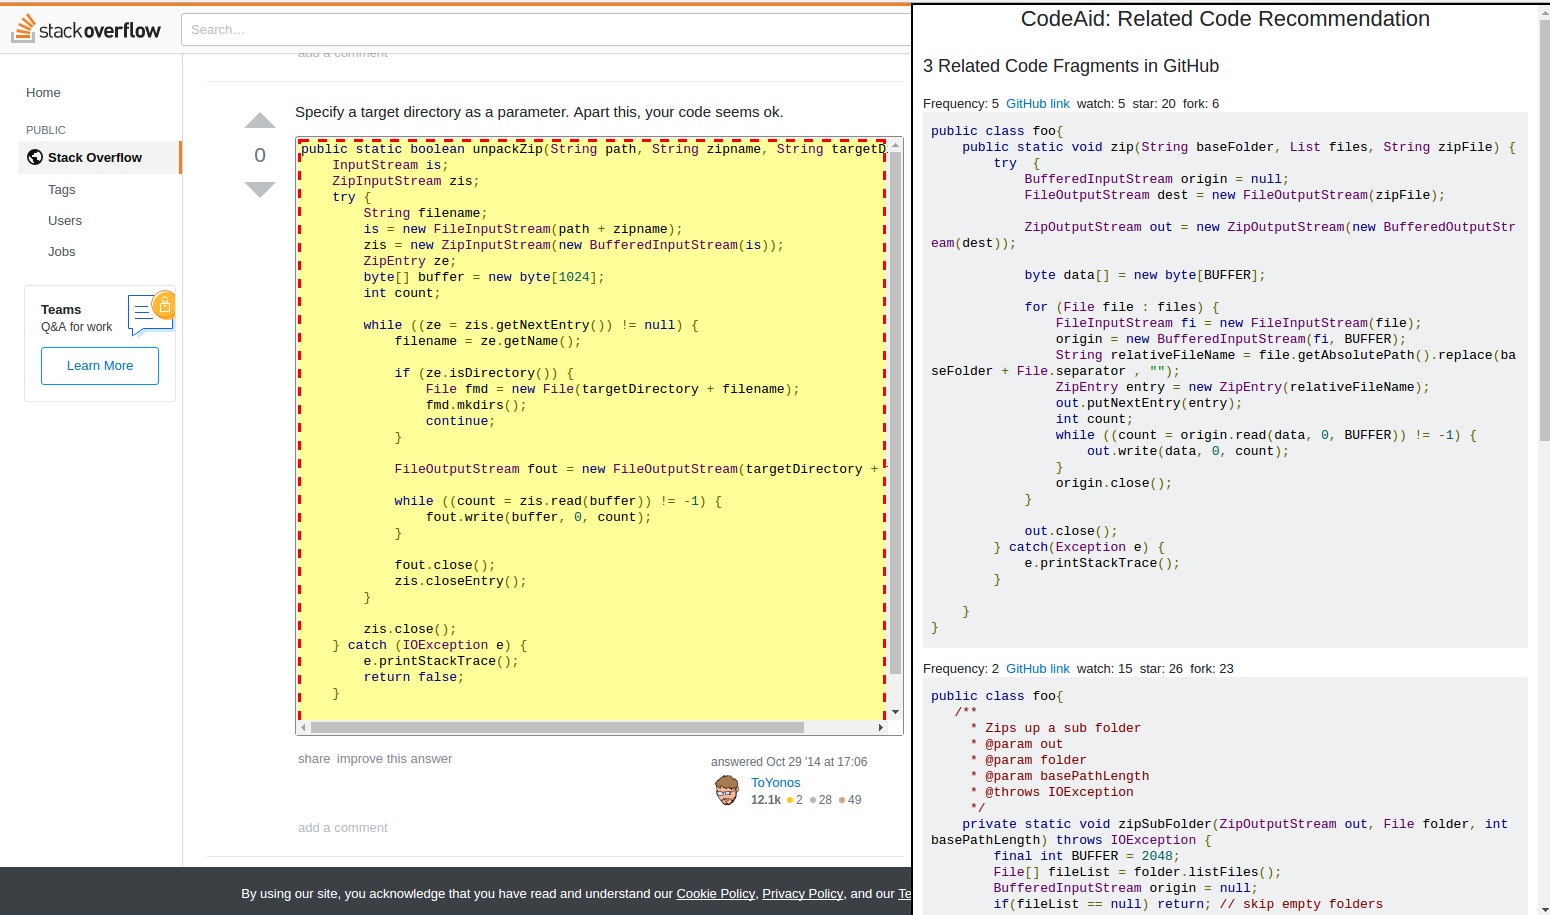
\includegraphics[width=\linewidth]{figures/ui.png}
	\caption{Screenshot of Chrome extension}
	\label{fig:chrome}
\end{figure*}